\section{Experiments \& Results}

\subsection{Part 1 Results: Hopper Continuous Control}

All three algorithms were trained for 70{,}000 episodes on the Hopper-v4 environment, repeated across three independent seeds.
Table~\ref{tab:part1_results} summarises the training performance;
Figure~\ref{fig:experiments_reward} shows the learning curves (rolling average over 100 episodes $\pm$ standard deviation across seeds).

In the table, \emph{Best Avg-100} is the peak value of the 100-episode rolling mean (averaged over seeds);
\emph{Final Avg-100} is the mean return over the last 100 training episodes; \emph{Std} is the standard deviation computed over all 70{,}000 episodes across all seeds;
\emph{Best Episode} is the highest single-episode return observed per seed, averaged across seeds;
\emph{Avg Ep.\ Len} is the mean episode length over the full 70{,}000 training episodes across all seeds;
\emph{Time (min)} is the total time required to train the agent.



\begin{table}[ht]
\centering
\caption{training performance on Hopper-v4 (mean over 3 seeds).}
\label{tab:part1_results}
\resizebox{\linewidth}{!}{%
\renewcommand{\arraystretch}{1.2}
\begin{tabular}{lrrrrcc}
\hline
\textbf{Algorithm} & \textbf{Best Avg-100} & \textbf{Final Avg-100} & \textbf{Std} & \textbf{Best Episode} & \textbf{Avg Ep.\ Len} & \textbf{Time (min)} \\
\hline
REINFORCE ($b{=}0$)  & 1006 & 635  & 257 & 2811 & 178 & 57.6 \\
REINFORCE ($b{=}20$) & 1807 & 806  & 399 & 3152 & 215 & 70.3 \\
Actor-Critic         & \textbf{1938} & \textbf{1360} & \textbf{734} & \textbf{3480} & \textbf{249} & \textbf{83.8} \\
\hline
\end{tabular}%
}
\end{table}

\begin{table}[ht]
\centering
\caption{test performance on Hopper-v4.}
\label{tab:part1_test_results}
\resizebox{\linewidth}{!}{%
\renewcommand{\arraystretch}{1.2}
\begin{tabular}{lccc}
\hline
\textbf{Algorithm} & \textbf{Seed} & \textbf{Test Return (Mean $\pm$ Std)} & \textbf{Test Length (Mean $\pm$ Std)} \\
\hline
REINFORCE ($b{=}0$)  & 1 & $710 \pm 484$ & $281 \pm 158$ \\
                     & 2 & $726 \pm 296$ & $230 \pm 85$ \\
                     & 3 & $1305 \pm 547$ & $582 \pm 283$ \\
\hline
REINFORCE ($b{=}20$) & 1 & $782 \pm 929$ & $304 \pm 350$ \\
                     & 2 & $1461 \pm 1097$ & $461 \pm 330$ \\
                     & 3 & $2444 \pm 182$ & $976 \pm 75$ \\
\hline
Actor-Critic         & 1 & $1725 \pm 1382$ & $555 \pm 432$ \\
                     & 2 & $\mathbf{3335 \pm 14}$ & $\mathbf{1000 \pm 0}$ \\
                     & 3 & $760 \pm 111$ & $251 \pm 30$ \\
\hline
\end{tabular}%
}
\end{table}

\begin{figure}[ht]
    \centering
    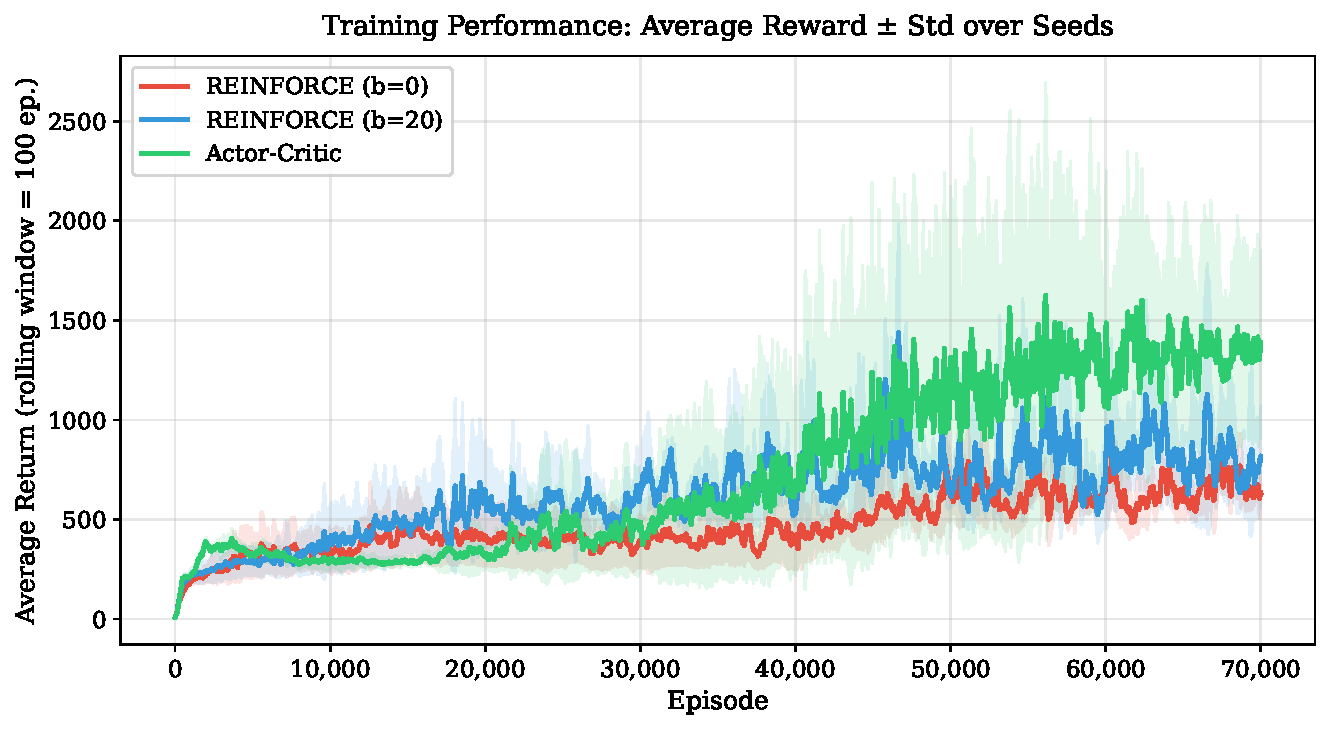
\includegraphics[width=\linewidth]{imgs/experiments_reward.pdf}
    \caption{Average return (rolling window $= 100$ episodes) $\pm$ standard deviation across 3 seeds for REINFORCE ($b{=}0$, $b{=}20$) and Actor-Critic on Hopper-v4.}
    \label{fig:experiments_reward}
\end{figure}

As we can clearly see from Table~\ref{tab:part1_results}, the Actor-Critic achieved the best overall training performance, outperforming the other models 
in terms of highest Best Avg-100 reward (1938), highest Final Avg-100 reward (1360), highest Best Episode reward (3480) and longest average episode length (249 steps).
In turn, REINFORCE with baseline achieved better overall scores than vanilla REINFORCE, improving the Best Avg-100 reward from 1006 to 1807 and the average
episode length from 178 to 215 steps.
Interestingly, despite expecting a gradient-estimator variance reduction with the introduction of a baseline, the opposite behaviour was recorded,
where REINFORCE with baseline exhibited a higher reward standard deviation (399 vs 257) than vanilla REINFORCE.

Figure~\ref{fig:experiments_reward} shows that the Hopper improved its policy throughout training under all algorithms.
However, the Actor-Critic achieved faster policy improvement, reaching larger reward quicker and eventually reaching reward scores that neither of the REINFORCE
variants were able to obtain.

The test results reported in Table~\ref{tab:part1_test_results} support the claim that the Actor-Critic outperformed the other approaches, although substantial variability
across seeds was recorded.
Indeed, the best Actor-Critic seed achieved a mean test return of $3335 \pm 14$ and consistently survived for the full episode ($1000 \pm 0$ steps).
On the other hand, the worst seed achieved a mere $760 \pm 111$ reward score, proving that Actor-Critic did not perform consistenlty across different seeds.
Lower scores but similar variability was observed for both REINFORCE variants.

Overall, the Actor-Critic performed the best both in training and testing among the evaluated methods.
Nevertheless, the large differences between seeds indicate that learning remained sensitive to initialization and stochastic training effects.












\subsection{Part 2 Results: PandaPush Sim-to-Sim Transfer}

Idea:
\begin{itemize}
    \item Show results of each algorithm $\Rightarrow$ SAC + UDR $\rightarrow$ SAC + ADR $\rightarrow$ SAC $\rightarrow$ PPO
    \item Reality gap $\Rightarrow$ vanilla SAC vs upper bound ; SAC + UDR vs upper bound
    \item Mass-sensitivity analysis $\Rightarrow$ vanilla SAC sucks and SAC + UDR achieves better results for general purpose
    \item Again, not sure about the correctness and pretty AI
\end{itemize}

\textbf{(Marco ha messo una tabella in report insights pt2 ma è gigantesca, inserirei separatamente le tabelle per i valori richiesti (Source-Source, Source-Target già fatta))}
\textbf{Risultati PPO per source-source: return -3.485 +- 0.091 sr 20\% +- 0.1, target->target solo su sac}

\begin{table}[h]
\centering
\begin{tabular}{lcc}
\hline
Method & Target Return & Target Success Rate \\ 
\hline
PPO & $-3.496 \pm 0.051$ & $20\% \pm 0.1\%$ \\
SAC (none) & $-0.633 \pm 0.152$ & $97.5\% \pm 0.3\%$ \\
SAC + ADR & $-0.556 \pm 0.044$ & $99.2\%$ \\
\textbf{SAC + UDR} & $\mathbf{-0.509 \pm 0.032}$ & $\mathbf{99.7\%}$ \\
Oracle & $-0.445 \pm 0.019$ & $100\%$ \\
\hline
\end{tabular}
\caption{Target-environment performance comparison.}
\label{table:target_performance}
\end{table}

The results clearly show that SAC outperforms PPO, both on source and training environments \ref{table:target_performance}. Even after an extensive hyperparameter tuning, PPO consistently plateaued around a return of -3.0 and failed to solve the task consistently (success rate:$\sim 20\%$). On the other hand, SAC successfully learned effective pushing policies and transferred well to the target environment.

Uniform Domain Randomization (UDR) achieved the best performance, outperforming both vanilla SAC and Automatic Domain Randomization (ADR). It achieved a target return of -0.509 compared to -0.556 for ADR and -0.633 for vanilla SAC. The policy obtained training directly on the target environment (oracle) achieved the best overall result (-0.445) but is not a valid sim-to-real solution because it has access to target dynamics during training, it only represents the upper bound.

The reality gap can be measured relative to the oracle.
\begin{itemize}
    \item The gap between vanilla SAC and the oracle is $(-0.445)-(-0.633)=0.188$.
    \item The gap between SAC + UDR and the oracle is $(-0.445)-(-0.509)=0.064$.
\end{itemize}

Therefore, the fraction of the gap removed by UDR is
\[
\frac{0.188-0.064}{0.188}=0.6596,
\]
corresponding to approximately 66\%.

This result indicates that UDR eliminates about two-thirds of the performance loss caused by the source-to-target mass shift.

Finally a mass-sensitivity analysis was conducted to further highlight the robustness gained thanks to domain randomization techniques. When evaluated at increasingly heavier masses, vanilla SAC deteriorates from -0.554 at 1 kg to -0.869 at 15 kg. In contrast, UDR only decreases from -0.478 to -0.592 over the same range. This demonstrates that UDR learns a policy that is robust across a wide range of dynamics rather than specialized to a single mass value.